\documentclass{article}
\usepackage[utf8]{inputenc}
\usepackage{hyperref}
\usepackage[letterpaper, portrait, margin=1in]{geometry}
\usepackage{enumitem}
\usepackage{amsmath}
\usepackage{booktabs}
\usepackage{graphicx}
\usepackage{longtable}
\usepackage{float}

\usepackage{hyperref}
\hypersetup{
colorlinks=true,
    linkcolor=black,
    filecolor=black,      
    urlcolor=blue,
    citecolor=black,
}
\usepackage{natbib}

\usepackage{titlesec}
  
\title{ECON 7103 Homework 8}
\author{Yifan Liu (yliu3494)}
\date{Spring 2023}
  
\begin{document}
  
\maketitle


\noindent
\\
1. The effect of the recycling pause and the possibility of parallel trends
\smallskip
\begin{figure}[H]
    \centering
    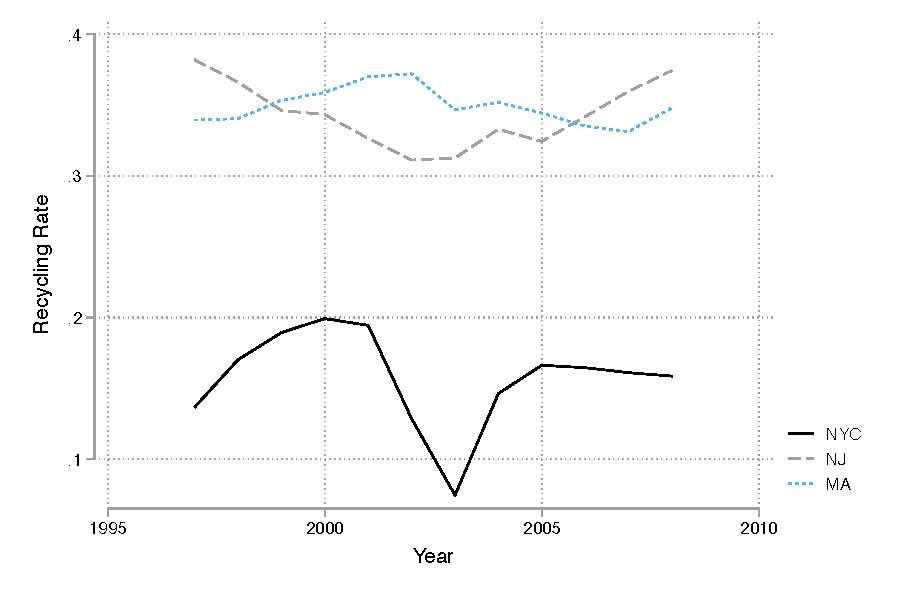
\includegraphics[scale = 0.7]{Q1.pdf}
    \caption{A yearly plot of the recycling rate for NYC and the controls}
    \label{fig:Q1}
\end{figure}
\noindent
\\ Figure 1 demonstrates a yearly plot of the recycling rate for NYC and the controls. There is a discernible drop of recycling rate between 2002 and 2004, which can result from the recycling pause. However, the trends between NYC and NJ or MA look quite different.
\bigskip

\noindent
\\
2. TWFE
\\ The average treatment effect of the recycling pause is -.06199 with a standard error of .0058.

\noindent
\\
3. Synthetic DID
\\ The average treatment effect of the recycling pause is -.06310 with a standard error of .03792.
\smallskip
\begin{figure}[H]
    \centering
    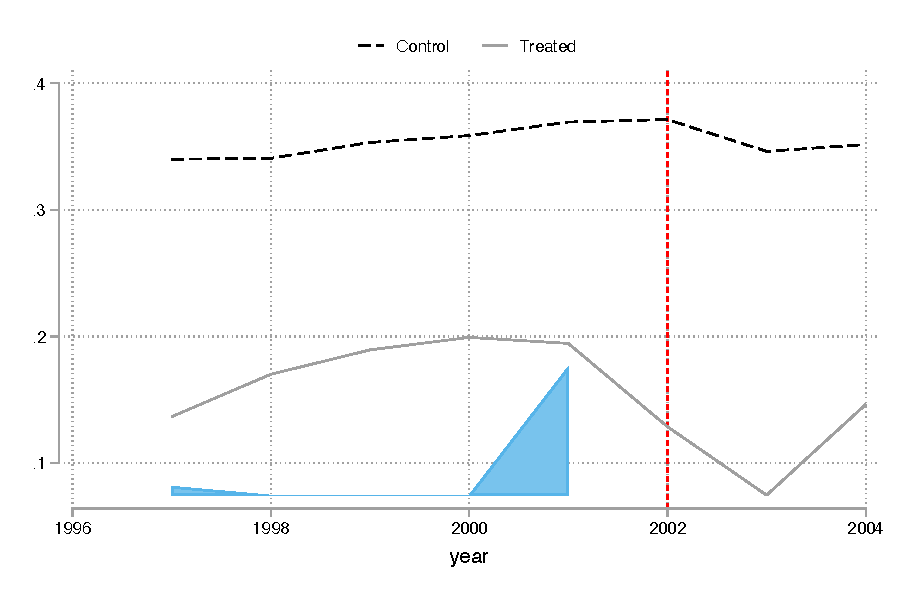
\includegraphics[scale = 0.7]{Q3.pdf}
    \caption{The synthetic DID plot}
    \label{fig:Q1}
\end{figure}

\noindent
\\
4. Event study
\\ Setting the year of 2001(dy5) as the benchmark, the effect of year 2002 (dy6) is -.06734 with a standard error of .0073.
\smallskip
\begin{figure}[H]
    \centering
    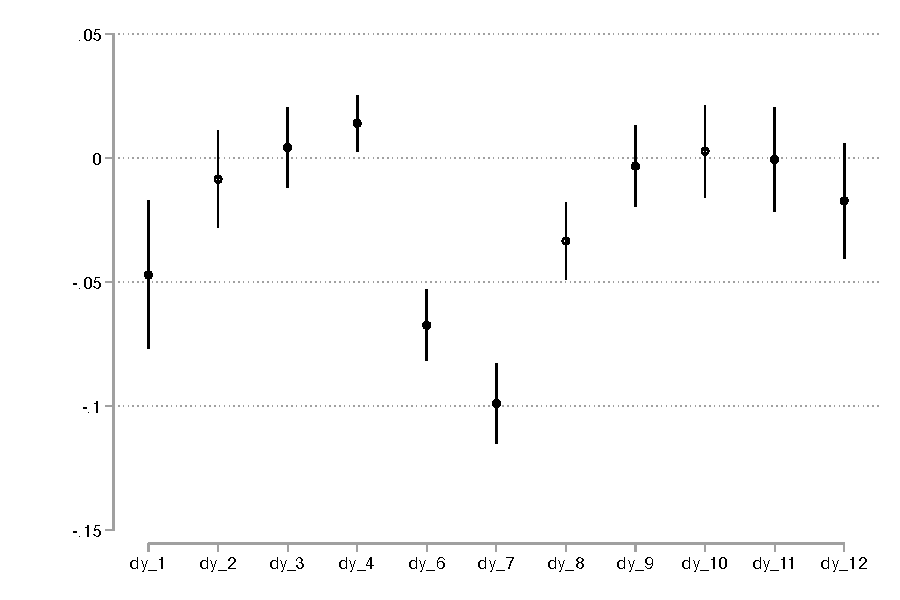
\includegraphics[scale = 0.7]{Q4.pdf}
    \caption{Event study}
    \label{fig:Q1}
\end{figure}

\noindent
\\
5. Synthetic control estimates
\bigskip
\\(a) The plot of raw outcomes for treated and control groups over time:
\smallskip
\begin{figure}[H]
    \centering
    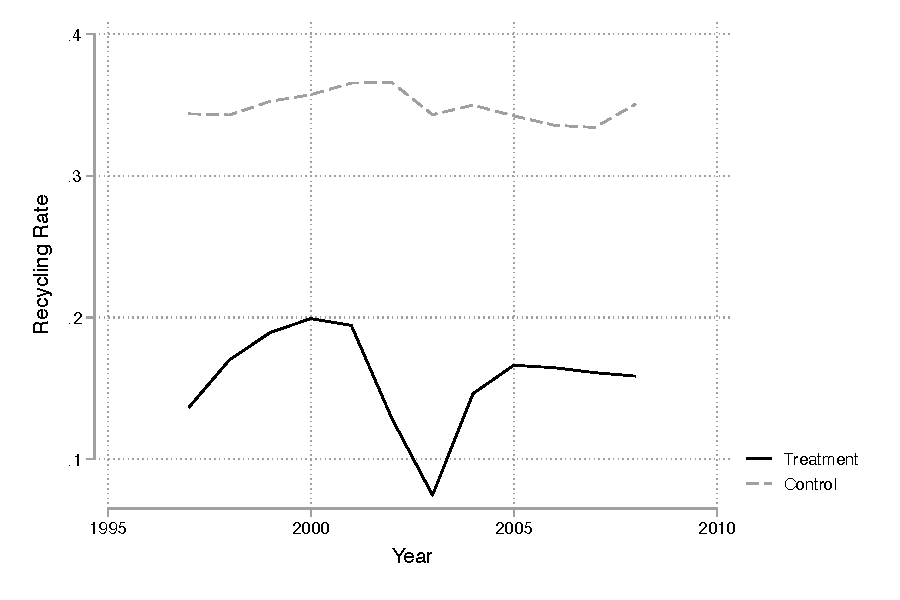
\includegraphics[scale = 0.7]{Q5a.pdf}
    \caption{Raw outcomes for treated and control groups over time (A)}
    \label{fig:Q5a}
\end{figure}
\smallskip
\begin{figure}[H]
    \centering
    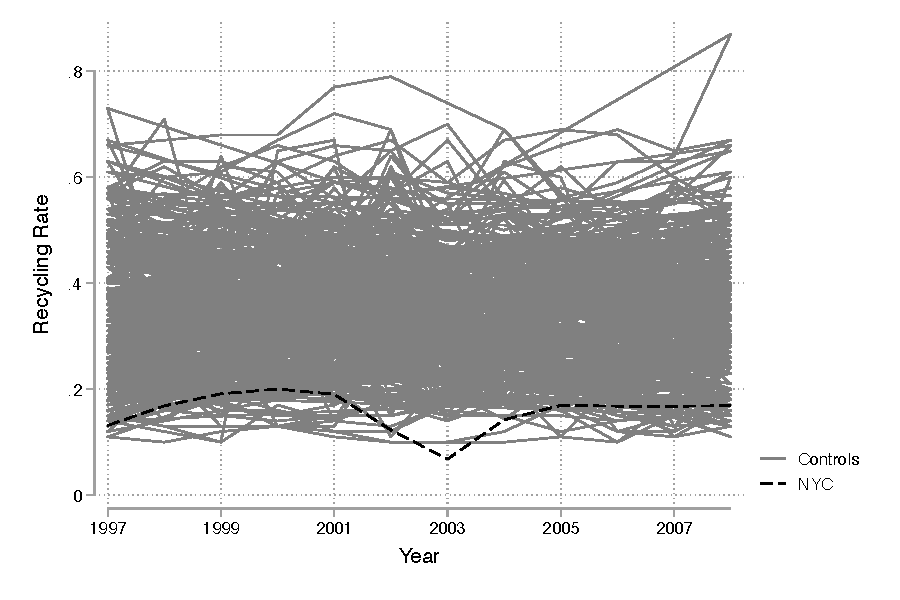
\includegraphics[scale = 0.7]{Q5aa.pdf}
    \caption{Raw outcomes for treated and control groups over time (B)}
    \label{fig:Q5aa}
\end{figure}
(b) The plot of raw outcomes for treated group and synthetic control group over time:
\smallskip
\begin{figure}[H]
    \centering
    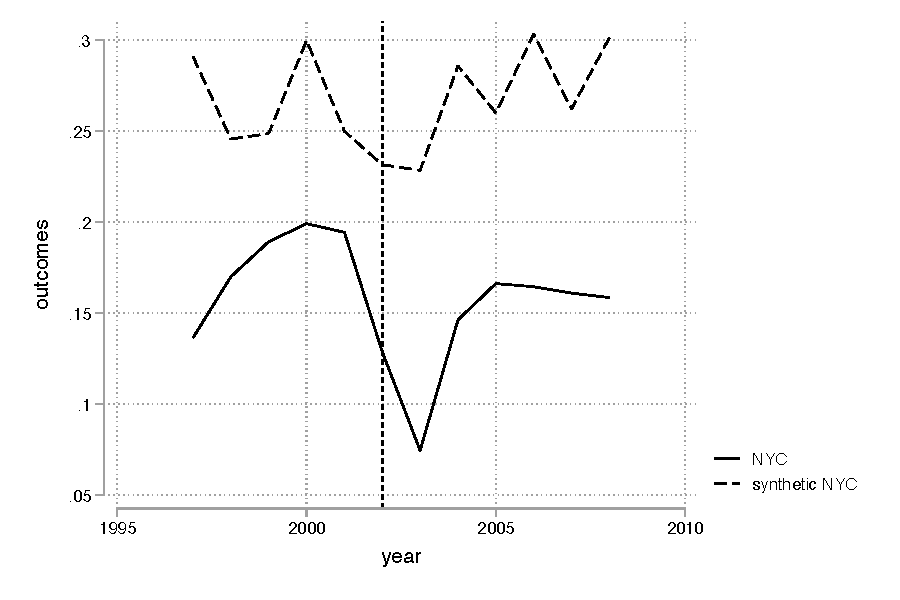
\includegraphics[scale = 0.7]{Q5b.pdf}
    \caption{Raw outcomes for treated group and synthetic control group over time}
    \label{fig:Q5b}
\end{figure}
(c) The plot of estimated synthetic control effects and placebo effects over time:
\smallskip
\begin{figure}[H]
    \centering
    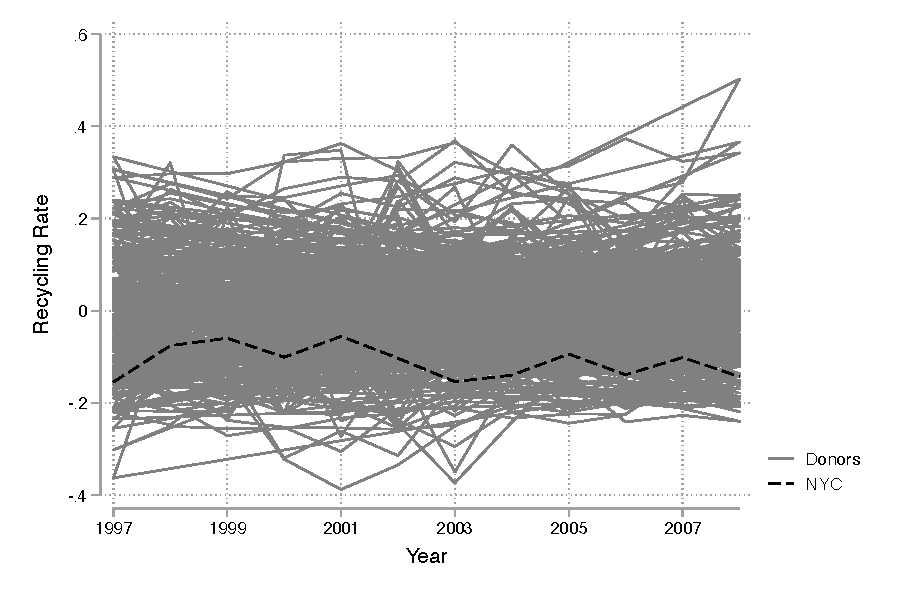
\includegraphics[scale = 0.7]{Q5c.pdf}
    \caption{Estimated synthetic control effects and placebo effects over time}
    \label{fig:Q5c}
\end{figure}
(d) The plot of final synthetic control estimates over time:
\smallskip
\begin{figure}[H]
    \centering
    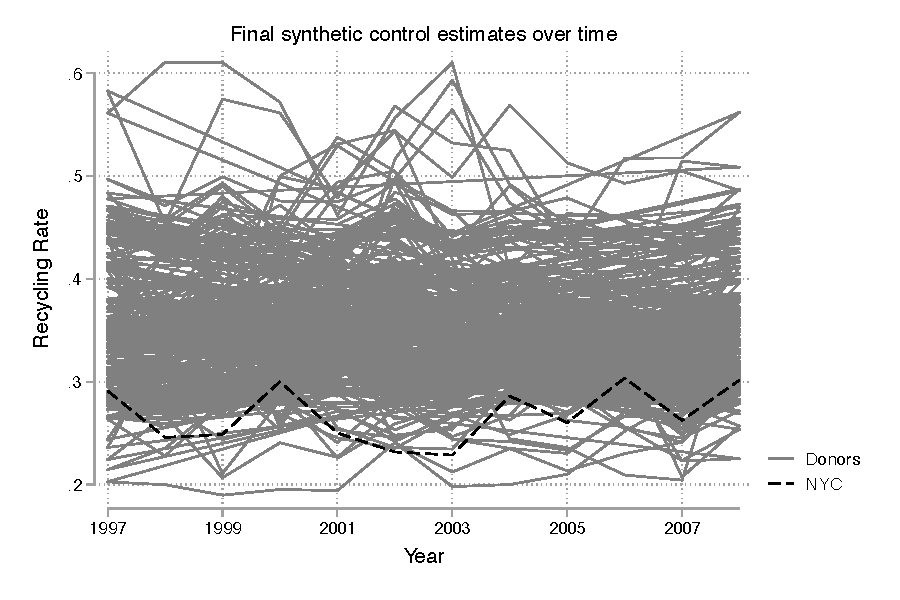
\includegraphics[scale = 0.7]{Q5d.pdf}
    \caption{Final synthetic control estimates over time}
    \label{fig:Q5d}
\end{figure}

\end{document}

